%% ODER: format ==         = "\mathrel{==}"
%% ODER: format /=         = "\neq "
%
%
\makeatletter
\@ifundefined{lhs2tex.lhs2tex.sty.read}%
  {\@namedef{lhs2tex.lhs2tex.sty.read}{}%
   \newcommand\SkipToFmtEnd{}%
   \newcommand\EndFmtInput{}%
   \long\def\SkipToFmtEnd#1\EndFmtInput{}%
  }\SkipToFmtEnd

\newcommand\ReadOnlyOnce[1]{\@ifundefined{#1}{\@namedef{#1}{}}\SkipToFmtEnd}
\usepackage{amstext}
\usepackage{amssymb}
\usepackage{stmaryrd}
\DeclareFontFamily{OT1}{cmtex}{}
\DeclareFontShape{OT1}{cmtex}{m}{n}
  {<5><6><7><8>cmtex8
   <9>cmtex9
   <10><10.95><12><14.4><17.28><20.74><24.88>cmtex10}{}
\DeclareFontShape{OT1}{cmtex}{m}{it}
  {<-> ssub * cmtt/m/it}{}
\newcommand{\texfamily}{\fontfamily{cmtex}\selectfont}
\DeclareFontShape{OT1}{cmtt}{bx}{n}
  {<5><6><7><8>cmtt8
   <9>cmbtt9
   <10><10.95><12><14.4><17.28><20.74><24.88>cmbtt10}{}
\DeclareFontShape{OT1}{cmtex}{bx}{n}
  {<-> ssub * cmtt/bx/n}{}
\newcommand{\tex}[1]{\text{\texfamily#1}}	% NEU

\newcommand{\Sp}{\hskip.33334em\relax}


\newcommand{\Conid}[1]{\mathit{#1}}
\newcommand{\Varid}[1]{\mathit{#1}}
\newcommand{\anonymous}{\kern0.06em \vbox{\hrule\@width.5em}}
\newcommand{\plus}{\mathbin{+\!\!\!+}}
\newcommand{\bind}{\mathbin{>\!\!\!>\mkern-6.7mu=}}
\newcommand{\rbind}{\mathbin{=\mkern-6.7mu<\!\!\!<}}% suggested by Neil Mitchell
\newcommand{\sequ}{\mathbin{>\!\!\!>}}
\renewcommand{\leq}{\leqslant}
\renewcommand{\geq}{\geqslant}
\usepackage{polytable}

%mathindent has to be defined
\@ifundefined{mathindent}%
  {\newdimen\mathindent\mathindent\leftmargini}%
  {}%

\def\resethooks{%
  \global\let\SaveRestoreHook\empty
  \global\let\ColumnHook\empty}
\newcommand*{\savecolumns}[1][default]%
  {\g@addto@macro\SaveRestoreHook{\savecolumns[#1]}}
\newcommand*{\restorecolumns}[1][default]%
  {\g@addto@macro\SaveRestoreHook{\restorecolumns[#1]}}
\newcommand*{\aligncolumn}[2]%
  {\g@addto@macro\ColumnHook{\column{#1}{#2}}}

\resethooks

\newcommand{\onelinecommentchars}{\quad-{}- }
\newcommand{\commentbeginchars}{\enskip\{-}
\newcommand{\commentendchars}{-\}\enskip}

\newcommand{\visiblecomments}{%
  \let\onelinecomment=\onelinecommentchars
  \let\commentbegin=\commentbeginchars
  \let\commentend=\commentendchars}

\newcommand{\invisiblecomments}{%
  \let\onelinecomment=\empty
  \let\commentbegin=\empty
  \let\commentend=\empty}

\visiblecomments

\newlength{\blanklineskip}
\setlength{\blanklineskip}{0.66084ex}

\newcommand{\hsindent}[1]{\quad}% default is fixed indentation
\let\hspre\empty
\let\hspost\empty
\newcommand{\NB}{\textbf{NB}}
\newcommand{\Todo}[1]{$\langle$\textbf{To do:}~#1$\rangle$}

\EndFmtInput
\makeatother
%
%
%
%
%
%
% This package provides two environments suitable to take the place
% of hscode, called "plainhscode" and "arrayhscode". 
%
% The plain environment surrounds each code block by vertical space,
% and it uses \abovedisplayskip and \belowdisplayskip to get spacing
% similar to formulas. Note that if these dimensions are changed,
% the spacing around displayed math formulas changes as well.
% All code is indented using \leftskip.
%
% Changed 19.08.2004 to reflect changes in colorcode. Should work with
% CodeGroup.sty.
%
\ReadOnlyOnce{polycode.fmt}%
\makeatletter

\newcommand{\hsnewpar}[1]%
  {{\parskip=0pt\parindent=0pt\par\vskip #1\noindent}}

% can be used, for instance, to redefine the code size, by setting the
% command to \small or something alike
\newcommand{\hscodestyle}{}

% The command \sethscode can be used to switch the code formatting
% behaviour by mapping the hscode environment in the subst directive
% to a new LaTeX environment.

\newcommand{\sethscode}[1]%
  {\expandafter\let\expandafter\hscode\csname #1\endcsname
   \expandafter\let\expandafter\endhscode\csname end#1\endcsname}

% "compatibility" mode restores the non-polycode.fmt layout.

\newenvironment{compathscode}%
  {\par\noindent
   \advance\leftskip\mathindent
   \hscodestyle
   \let\\=\@normalcr
   \let\hspre\(\let\hspost\)%
   \pboxed}%
  {\endpboxed\)%
   \par\noindent
   \ignorespacesafterend}

\newcommand{\compaths}{\sethscode{compathscode}}

% "plain" mode is the proposed default.
% It should now work with \centering.
% This required some changes. The old version
% is still available for reference as oldplainhscode.

\newenvironment{plainhscode}%
  {\hsnewpar\abovedisplayskip
   \advance\leftskip\mathindent
   \hscodestyle
   \let\hspre\(\let\hspost\)%
   \pboxed}%
  {\endpboxed%
   \hsnewpar\belowdisplayskip
   \ignorespacesafterend}

\newenvironment{oldplainhscode}%
  {\hsnewpar\abovedisplayskip
   \advance\leftskip\mathindent
   \hscodestyle
   \let\\=\@normalcr
   \(\pboxed}%
  {\endpboxed\)%
   \hsnewpar\belowdisplayskip
   \ignorespacesafterend}

% Here, we make plainhscode the default environment.

\newcommand{\plainhs}{\sethscode{plainhscode}}
\newcommand{\oldplainhs}{\sethscode{oldplainhscode}}
\plainhs

% The arrayhscode is like plain, but makes use of polytable's
% parray environment which disallows page breaks in code blocks.

\newenvironment{arrayhscode}%
  {\hsnewpar\abovedisplayskip
   \advance\leftskip\mathindent
   \hscodestyle
   \let\\=\@normalcr
   \(\parray}%
  {\endparray\)%
   \hsnewpar\belowdisplayskip
   \ignorespacesafterend}

\newcommand{\arrayhs}{\sethscode{arrayhscode}}

% The mathhscode environment also makes use of polytable's parray 
% environment. It is supposed to be used only inside math mode 
% (I used it to typeset the type rules in my thesis).

\newenvironment{mathhscode}%
  {\parray}{\endparray}

\newcommand{\mathhs}{\sethscode{mathhscode}}

% texths is similar to mathhs, but works in text mode.

\newenvironment{texthscode}%
  {\(\parray}{\endparray\)}

\newcommand{\texths}{\sethscode{texthscode}}

% The framed environment places code in a framed box.

\def\codeframewidth{\arrayrulewidth}
\RequirePackage{calc}

\newenvironment{framedhscode}%
  {\parskip=\abovedisplayskip\par\noindent
   \hscodestyle
   \arrayrulewidth=\codeframewidth
   \tabular{@{}|p{\linewidth-2\arraycolsep-2\arrayrulewidth-2pt}|@{}}%
   \hline\framedhslinecorrect\\{-1.5ex}%
   \let\endoflinesave=\\
   \let\\=\@normalcr
   \(\pboxed}%
  {\endpboxed\)%
   \framedhslinecorrect\endoflinesave{.5ex}\hline
   \endtabular
   \parskip=\belowdisplayskip\par\noindent
   \ignorespacesafterend}

\newcommand{\framedhslinecorrect}[2]%
  {#1[#2]}

\newcommand{\framedhs}{\sethscode{framedhscode}}

% The inlinehscode environment is an experimental environment
% that can be used to typeset displayed code inline.

\newenvironment{inlinehscode}%
  {\(\def\column##1##2{}%
   \let\>\undefined\let\<\undefined\let\\\undefined
   \newcommand\>[1][]{}\newcommand\<[1][]{}\newcommand\\[1][]{}%
   \def\fromto##1##2##3{##3}%
   \def\nextline{}}{\) }%

\newcommand{\inlinehs}{\sethscode{inlinehscode}}

% The joincode environment is a separate environment that
% can be used to surround and thereby connect multiple code
% blocks.

\newenvironment{joincode}%
  {\let\orighscode=\hscode
   \let\origendhscode=\endhscode
   \def\endhscode{\def\hscode{\endgroup\def\@currenvir{hscode}\\}\begingroup}
   %\let\SaveRestoreHook=\empty
   %\let\ColumnHook=\empty
   %\let\resethooks=\empty
   \orighscode\def\hscode{\endgroup\def\@currenvir{hscode}}}%
  {\origendhscode
   \global\let\hscode=\orighscode
   \global\let\endhscode=\origendhscode}%

\makeatother
\EndFmtInput
%
%
%
% First, let's redefine the forall, and the dot.
%
%
% This is made in such a way that after a forall, the next
% dot will be printed as a period, otherwise the formatting
% of `comp_` is used. By redefining `comp_`, as suitable
% composition operator can be chosen. Similarly, period_
% is used for the period.
%
\ReadOnlyOnce{forall.fmt}%
\makeatletter

% The HaskellResetHook is a list to which things can
% be added that reset the Haskell state to the beginning.
% This is to recover from states where the hacked intelligence
% is not sufficient.

\let\HaskellResetHook\empty
\newcommand*{\AtHaskellReset}[1]{%
  \g@addto@macro\HaskellResetHook{#1}}
\newcommand*{\HaskellReset}{\HaskellResetHook}

\global\let\hsforallread\empty

\newcommand\hsforall{\global\let\hsdot=\hsperiodonce}
\newcommand*\hsperiodonce[2]{#2\global\let\hsdot=\hscompose}
\newcommand*\hscompose[2]{#1}

\AtHaskellReset{\global\let\hsdot=\hscompose}

% In the beginning, we should reset Haskell once.
\HaskellReset

\makeatother
\EndFmtInput
















%%format ._ = "."








\begin{figure*}[t]
  \begin{center}
  \fbox{
        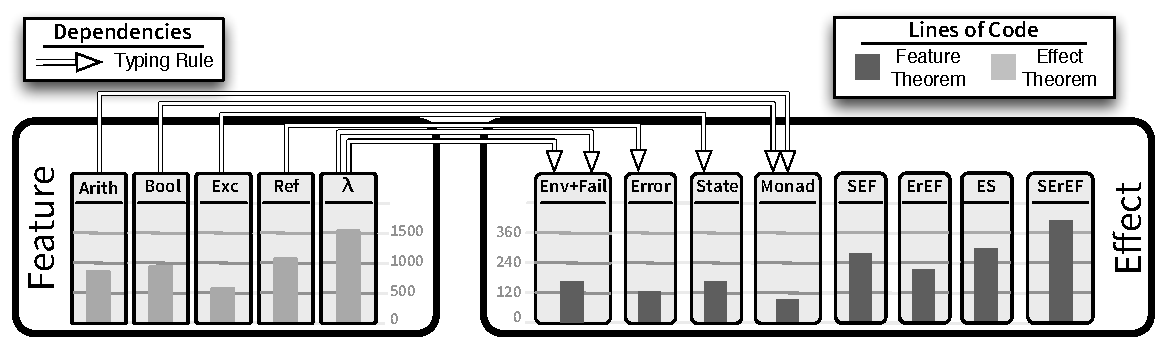
\includegraphics[scale = .85]{src/ModularEffects/CaseStudyFigure.pdf}
   }
  \end{center}
  \caption{Dependency and size information for the features and effects used in the case study.}
  \label{fig:codesize}
\end{figure*}

\section{Case Study}
\label{sec:CaseStudy}

As a demonstration of the \Name~framework, we have built a set of five
reusable language features and combined them to build a family of
languages which includes a mini-ML~\cite{clement86mini-ML} variant
with references and errors. The study includes pure boolean and
arithmetic features as well as effectful features for references,
errors and lambda abstractions.

The study builds twenty eight different combinations of the features which are
all possible combinations with at least one feature providing
values.\footnote{Also available at \url{http://www.cs.utexas.edu/~bendy/3MT}}
Figure~\ref{fig:MiniMLSyntax} presents the syntax of the expressions,
values, and types provided; each line is annotated with the feature
that provides that set of definitions.

Four kinds of feature interactions appear in the case study.

\begin{itemize}

\item The PHOAS representation of binders requires an auxiliary
equivalence relation, the details of which are covered in the MTC
paper~\cite{mtc}. The soundness proofs of language theorems for
languages which include binders proceed by induction over this
equivalence relation instead of expressions. The reusable feature
theorems of other features need to be lifted to this equivalence
relation.

\item The effect theorems that feature an environment
typing $\Sigma$, such as those for state or environment, need a weakening sublemma
which
states
that each well-formed value under
$\Sigma$ is also well-formed under a conservative extension:
\[\Sigma \vdash v ~:~ t  \\ \rightarrow \\
  \Sigma' \supseteq \Sigma \\ \rightarrow \\
  \Sigma' \vdash v ~:~ t \]
\item Inversion lemmas for the well-formed value relation as in the
proof of \ref{thm:FSound} for the boolean feature in
Section \ref{sec:Thm+Reuse} are proven by induction over the
relation.

%% \item The sublemmas of reusable feature theorems for properties such as
%% \textsc{WFM-If-Vc} are
%% proven by induction over the extensible typing relation. When effectful
%% features introduce new judgements to the relation, these new
%% judgements must have proof algebra instances for the sublemmas.

\end{itemize}


The proofs of the first and second kind of feature interactions are
straightforward; the inversion lemmas of the third kind can be
dispatched by tactics hooked into the type class inference algorithm.
%% The last kind of interactions require more work and comprise the
%% biggest part of the code dealing with feature interactions.
%%
%% The presented typing rules for effects satisfy the \textsc{WFM-Bind}
%% property; as previously discussed, it can be used cut down on feature
%% interactions. The lambda feature uses \textsc{WFM-Bind} in its proof
%% of \ref{thm:FSound} instead of targeted sublemmas. The following table
%% shows the number of sublemmas used by the reusable feature theorems,
%% highlighting that the \textsc{WFM-Bind} property provides significantly
%% more convenience despite its stronger assumptions.


The framework itself consists of about 4,400 LoC of which about 2,000
LoC comprise the implementation of the monad transformers and their
algebraic laws. The size in LoC of the implementation of semantic
evaluation and typing functions and the reusable feature theorem for
each language feature is given in the left box in Figure
\ref{fig:codesize}. The right box lists the sizes of the effect
theorems. Each language needs on average 110 LoC to assemble its
semantic functions and soundness proofs from those of its features and
the effect theorem for its set of effects.


\begin{figure}[t]
  \begin{center}
    \begin{minipage}{\columnwidth}
      \begin{center}
        \fbox{
        \hspace{-.3cm}
          \begin{tabular}{r@{~}c@{~}lr}
            {\tt e} & ::= & {\tt $\mathbb{N}$ $|$ e + e} & \textit{Arith}\\
            & $|$ &  {\tt $\mathbb{B}$ $|$ {\bf if} e {\bf then} e {\bf else} e} & \textit{Bool} \\
           %% & $|$ & {\tt {\bf case} e {\bf of \{ z} $\Rightarrow$ e $\mathbf{;}$ {\bf S} n $\Rightarrow$ e\}} & \textit{NatCase}\\
            & $|$ & {\tt {\bf lam} x : T.e $|$ e e $|$ x} & \textit{Lambda}\\
            & $|$ & {\tt {\bf ref} e $|$ !e $|$ e:=e} & \textit{References}\\
            & $|$ & {\tt {\bf try} e {\bf with} e} $|$ {\bf error} & \textit{Errors}\\
           %%  & $|$ & {\tt {\bf fix} x : T.e} & \textit{Recursion}\\
          \end{tabular}
        }
      \end{center}
    \end{minipage}
    \begin{minipage}{\columnwidth}
      \hspace{-.3cm}
    \begin{tabular}{cc}
      \begin{minipage}{.48\columnwidth}
        \fbox{
        \hspace{-.3cm}
          \begin{tabular}{r@{~}c@{~}lr}
            {\tt V} & ::= & {\tt $\mathbb{N}$} & \textit{Arith}\\
            & $|$ &  {\tt $\mathbb{B}$} & \textit{Bool} \\
            & $|$ & {\tt {\bf clos} e $\mathtt{\overline{V}}$} & \textit{Lambda}\\
            & $|$ & {\tt {\bf loc} $\mathbb{N}$} & \textit{References}\\
          \end{tabular}
        }
      \end{minipage} &
      \begin{minipage}{.38\columnwidth}
        \hspace{-.3cm}
        \fbox{
        \hspace{-.3cm}
          \begin{tabular}{r@{~}c@{~}lr}
            {\tt T} & ::= & {\tt \bf Nat} & \textit{Arith}\\
            & $|$ &  {\tt \bf Bool} & \textit{Bool} \\
            & $|$ & {\tt T $\rightarrow$ T} & \textit{Lambda}\\
            & $|$ & {\tt {\bf Ref} T} & \textit{References}\\
          \end{tabular}
        }
      \end{minipage}
    \end{tabular}
    \end{minipage}
  \end{center}
  \caption{mini-ML expressions, values, and types}
  \label{fig:MiniMLSyntax}
\end{figure}


%% \begin{center}
%%   \fbox{
%%   \hspace{-.3cm}
%%     \begin{tabular}{ c c c c c }
%%       \textit{Arith} & \textit{Bool} & \textit{Errors} & \textit{References} & \textit{Lambda} \\
%%       2 & 3 & 0 & 4 & 0 \\
%%     \end{tabular}
%%   }
%% \end{center}
%% Each sublemma of the above table requires on average 50 LoC per effect.
